% Mode-matched record horizons in reversible dynamics — SciPost Physics submission draft
% Compile: latexmk -pdf main   (REVTeX 4.2; figures pulled from ../figures/)
\documentclass[aps,pre,twocolumn,superscriptaddress,nofootinbib,longbibliography]{revtex4-2}

\usepackage{graphicx}
\usepackage{amsmath,amssymb}
\usepackage{bm}
\usepackage[colorlinks=true,linkcolor=blue,citecolor=blue,urlcolor=blue]{hyperref}
\graphicspath{{../figures/}}

\newcommand{\tS}{t_{\mathrm{S}}}
\newcommand{\tstar}{t^{*}}
\newcommand{\Smax}{S_{\max}}
\newcommand{\kap}{\kappa}

\begin{document}

\title{Mode-matched record horizons in reversible dynamics:\\
relaxation, redundancy, and protected exceptions}

\author{Juneyoung Kim}
\email{lpaiu-cs@gmail.com}
\affiliation{Independent Researcher}

\date{\today}

\begin{abstract}
In the standard account of the arrow of time the memory arrow is slaved to the
thermodynamic gradient: records form on the entropy-increasing side of a low-entropy
boundary condition. Here we quantify record-keeping itself. In an exactly bit-reversible
lattice gas we place two clocks on the same runs: the entropy-saturation time $\tS$
(coarse-grained entropy reaches $0.9\,\Smax$) and an \emph{operational record horizon}
$\tstar$, the time at which an explicit held-out linear readout of the present coarse state
retains less than half a bit about a planted macroscopic fact. For boundary-scale records
we find $\tstar=\kap\,\tS$ with $\kap$ of order one and flat across scrambling rates
($\kap=1.08$ over a $7\times$ range) and system sizes ($\bar\kap=0.99$, $L=48$--$128$); the
same proportionality reproduces in a continuous hard-disk gas ($\kap=1.00$) and in exactly
reversible Clifford circuits of up to $128$ qubits ($\kap=0.79$), and survives a
Haar-random (non-Clifford) control. A one-slow-mode analysis accounts for the law: entropy
deficit and record signal relax on a shared timescale, so both crossings take the form
$\tau\ln(A/\theta)$ and $\kap$ is a ratio of logarithms; the reconstruction has no
additional free parameters (median error $5\%$/$1\%$) and predicts held-out runs at
comparable accuracy. The analysis' sharper consequence is confirmed by making the record's
wavelength an independent knob: the entropy clock is unchanged ($\tS$ varies by $2\%$)
while the horizon spans $9\times$, each mode's lifetime given by its own
$\tau_M\ln(A_M/\theta)$ to $1$--$5\%$. \emph{A record lives as long as the mode that
carries it}; among relaxing records the longest horizons are of order the thermalization
time, attained at the boundary scale, while a non-relaxing mode escapes the clock
entirely. The law fails exactly where it must---an engineered conservation law decouples
$\tstar$ from $\tS$, and one of $25$ lattice realizations does the same
\emph{spontaneously}, storing its record in a diagnosed frozen cluster at full fidelity
for $48\,\tS$---and records are stored redundantly,
with effective redundancy growing as $N^{\alpha}$, $\alpha_\infty=0.92\pm0.04$
(conservative) classically and $\alpha=1$ for quantum broadcast states. These results
quantify the sense in which the recorded past is the direction of the entropy
gradient---while leaving the low-entropy boundary itself unexplained.
\end{abstract}

\maketitle

\section{Introduction}
\label{sec:intro}

Microscopic dynamics---classical Hamiltonian flow, unitary quantum evolution, or the exactly
bit-reversible cellular automata used below---has no arrow of time. The observed asymmetry is
standardly traced to a low-entropy boundary condition (the Past Hypothesis) together with
coarse-graining \cite{boltzmann1877,lebowitz1993,albert2000,price1996,penrose1979}. Within
this picture the \emph{memory} (or ``psychological'') arrow is derivative: a physical record
is a present macrostate correlated with a macrostate at another time, and such correlations
are abundant only on the entropy-increasing side of the boundary
\cite{reichenbach1956,wolpert1992,mlodinowbrun2014,rovelli2020memory,halliwell1999,gellmannhartle1993}.
Reichenbach's fork asymmetry, Wolpert's analysis of memory systems, and Mlodinow and Brun's
argument that a robust record-forming system must sit on the entropy-increasing side all
support the same conclusion: \emph{memory points down the entropy gradient}.

The quantitative structure of record-keeping is less settled. Rovelli has argued that
individual memories degrade as the memory system thermalizes \cite{rovelli2020memory};
Riedel, Zurek, and Zwolak showed that relaxation toward equilibrium destroys the
\emph{redundancy} of environmental records in decoherence models \cite{riedel2012risefall};
and the quantum Darwinism program
\cite{zurek2003rmp,zurek2009darwinism,ollivier2004,blumekohout2006} identified redundant
imprinting as what makes a fact objective while it lasts. Observational entropy
\cite{safranek2019a,safranek2019b,safranek2021intro,strasberg2021} supplies the bookkeeping
for coarse observers of closed systems, and its increase has recently been shown to be
generic in isolated systems \cite{nagasawa2024}. What these threads have not provided is a
controlled, same-run comparison of a record's operational lifetime against the
thermodynamic clock of the same dynamics; a test of \emph{what} sets that lifetime when the
record's spatial structure is varied; and the boundary of the resulting law---the regime in
which it demonstrably fails.

This paper reports such measurements. Our testbed is deliberately minimal: exactly
reversible model dynamics (a Margolus block cellular automaton
\cite{margolus1984,toffolimargolus1987}, an event-driven hard-disk gas, and Clifford
circuits \cite{gottesman1998,aaronsongottesman2004}), a coarse-grained Boltzmann entropy,
and a one-bit macroscopic fact planted at the low-entropy boundary whose readability we
track with an explicit decoder. Our contributions:

\begin{enumerate}
\item \textbf{Bookkeeping} (Sec.~\ref{sec:setup}): over an ensemble of microstates evolved
by a bijective map, the fine-grained (Gibbs/Shannon) entropy is conserved to machine
precision while the observational entropy rises; the rise is \emph{identically} the growth
of information hidden from the coarse observer, $\Delta S_{\mathrm{obs}}=\Delta I$. In
parallel runs, a planted record decays to zero as the same coarse description saturates.
\item \textbf{A horizon law for boundary-scale records} (Sec.~\ref{sec:horizon}): the
record horizon tracks the entropy-saturation time, $\tstar=\kap\,\tS$ with $\kap$ order
one, flat across scrambling rates ($7\times$ in $\tS$) and system sizes.
\item \textbf{A one-slow-mode account} (Sec.~\ref{sec:mechanism}): entropy deficit and
record signal decay exponentially on a shared timescale, making both crossings
$\tau\ln(A/\theta)$ and $\kap$ a ratio of logarithms. The account reconstructs the measured
crossings with no additional free parameters (median error $5\%$/$1\%$) and predicts
held-out runs out-of-sample at comparable accuracy.
\item \textbf{The mode-resolved law} (Sec.~\ref{sec:modes}): making the record's wavelength
an independent knob shows the general statement is \emph{mode-matched}: the entropy clock
does not care which record was planted ($\tS$ flat to $2\%$) while the horizon spans
$9\times$, each mode's lifetime reproduced by its own $\tau_M\ln(A_M/\theta)$ to
$1$--$5\%$. ``Record lifetime $=$ thermalization time'' is the \emph{supremum} of this
law over relaxing records, attained by those written in the slowest mode.
\item \textbf{Cross-substrate corroboration} (Sec.~\ref{sec:universality}): the
boundary-scale proportionality reproduces in a continuous hard-disk gas and in reversible
Clifford circuits (up to $N=128$ qubits), and survives a Haar-random statevector control.
\item \textbf{A falsification boundary} (Sec.~\ref{sec:falsification}): the law is
contingent on ergodicity. A conservation law protecting the record makes $\tstar$ diverge
while $\tS$ stays finite---the extreme case of a non-relaxing mode.
\item \textbf{Redundancy scaling} (Sec.~\ref{sec:redundancy}): near the boundary the record
is recoverable from any $\sim1/8$ of the environment (effective redundancy
$R_\delta\approx8$--$10$); $R_\delta$ grows with the number of environment fragments as
$N^{\alpha}$ with a conservative $\alpha_\infty=0.92\pm0.04$, while a quantum broadcast
realizes ideal Darwinism, $\alpha=1$ exactly---consistent with the classical shortfall
being a signal-to-noise and finite-size effect rather than a limit of the principle.
\end{enumerate}

Throughout we are explicit about scope and about what is \emph{not} shown
(Sec.~\ref{sec:discussion}): the low-entropy boundary is an input, as it must be for any
time-symmetric dynamics \cite{loschmidt1876}; $\tstar$ is an operational,
decoder-relative quantity (a lower bound on the accessible-information horizon), and the
numerical value of $\kap$ is convention-dependent---the physics is the shared relaxation
and its mode structure. All code, the scripts generating every figure, and per-run data
for the core experiments are public \cite{repo}.

\section{Setup: substrates, records, and bookkeeping}
\label{sec:setup}

\subsection{Reversible substrates and coarse entropy}

Our primary substrate is a Margolus block cellular automaton
\cite{margolus1984,toffolimargolus1987}: a two-dimensional lattice gas on an $L\times L$
grid of binary site occupations, updated in $2\times2$ blocks by bijective lookup tables
with alternating block offsets. A quenched random fraction (``scatter'') of blocks applies a
rotation rule, breaking spurious conservation laws so the gas thermalizes cleanly; the map
remains exactly bijective, and the inverse map recovers the initial bitstring exactly
(verified bit-for-bit \cite{repo}). Appendix~\ref{app:model} gives details. Two companion
substrates are used for universality tests: an event-driven hard-disk gas (elastic disks,
specular walls; exact between-collision flight) and Clifford brickwork circuits simulated in
the stabilizer formalism (Appendix~\ref{app:stabilizer}).

The coarse-grained (Boltzmann) entropy is defined by partitioning the grid into $b\times b$
cells and counting microstates compatible with the cell occupancies $\{n_i\}$:
\begin{equation}
S \;=\; \sum_i \ln \binom{b^2}{n_i},
\label{eq:boltzS}
\end{equation}
with $\Smax$ its microcanonical maximum at the given particle number. Initial states are
low-entropy ``blobs'': all particles confined to a region of width $w$ at density $\rho$,
with microstates drawn microcanonically within the blob.

\subsection{Records and the two clocks}

A \emph{record} is operationalized as follows. A one-bit macroscopic fact $F$ (in the
baseline construction, a marker of identical particle number placed on the left or the
right side of the blob, so the two classes differ in no conserved quantity) is planted at
$t=0$. For each class we evolve an ensemble of $K$ microstates through the same quenched
disorder. The readout at time $t$ is a nearest-centroid \emph{linear} decoder $\hat F$
trained on the coarse occupancy vectors of half of the worlds and evaluated on the held-out
half; the accessible record is the mutual information $I(F;\hat F)$ estimated from the
held-out confusion matrix (Appendix~\ref{app:decoder}). This is a
\emph{present-macrostate} readout: the decoder sees only the coarse state at time $t$,
never the history.

Two caveats define the scope of $\tstar$. First, it is \emph{operational}: a particular
readout's horizon, hence a lower bound on the horizon of the full accessible information
$I(F;\text{coarse state})$. Section~\ref{sec:modes} quantifies the readout dependence: at
the slowest mode three different readouts (trained linear, untrained fixed-template,
debiased Gaussian plug-in) agree to within the logarithmic threshold offsets the mechanism
predicts, while non-adaptive readouts of \emph{drifting} fine-scale patterns lose the
record earlier for physical reasons. Second, the thresholds below are conventions;
Sec.~\ref{sec:mechanism} shows crossings depend on them only logarithmically, and the
time-rescaled collapses make the convention-independent content explicit.

The two clocks, defined on the same runs:
\begin{align}
\tS &: \quad \text{first time } S(t) \ge 0.9\,\Smax,
\label{eq:tS}\\
\tstar &: \quad \text{first time } I(F;\hat F) < \tfrac12~\text{bit}.
\label{eq:tstar}
\end{align}

\subsection{Bookkeeping: the ledger identity}

Before measuring lifetimes we fix the bookkeeping. Consider an ensemble of $K$ equiprobable
microstates evolved by the (bijective) dynamics. The Shannon entropy $H$ of the microstate
distribution is exactly conserved, $H=\ln K$; in our runs ($K=64$, $L=128$, $T=2400$ steps)
the deviation is zero to machine precision, $\max_t|H-\ln K|=0$. The observational entropy
\cite{safranek2019a,safranek2019b} of the coarse observer decomposes as
\begin{equation}
S_{\mathrm{obs}}(t) \;=\; H \;+\; I(t), \qquad I(t)\ge 0,
\label{eq:ledger}
\end{equation}
where $I(t)$ is the information about the microstate hidden from the coarse observer
(Appendix~\ref{app:decoder}). Equation~\eqref{eq:ledger} is an identity of the
coarse-graining, not an empirical finding; its content here is that $H$ is exactly constant
under the bijective dynamics, so \emph{all} growth of $S_{\mathrm{obs}}$ is growth of the
hidden-information term (Fig.~\ref{fig:ledger}, left). In parallel runs of the same
substrate class ($K=64$, $L=64$), a planted record decays from $1.000$ bit to $0.006$ bit
as the coarse entropy saturates (Fig.~\ref{fig:ledger}, right). We present these as two
faces of one coarse-graining---the observer's global ignorance grows while its grip on any
planted fact decays---without claiming a computed decomposition of $I(t)$ into
record-specific parts; the quantitative link between the two clocks is the subject of the
rest of the paper.

\begin{figure*}
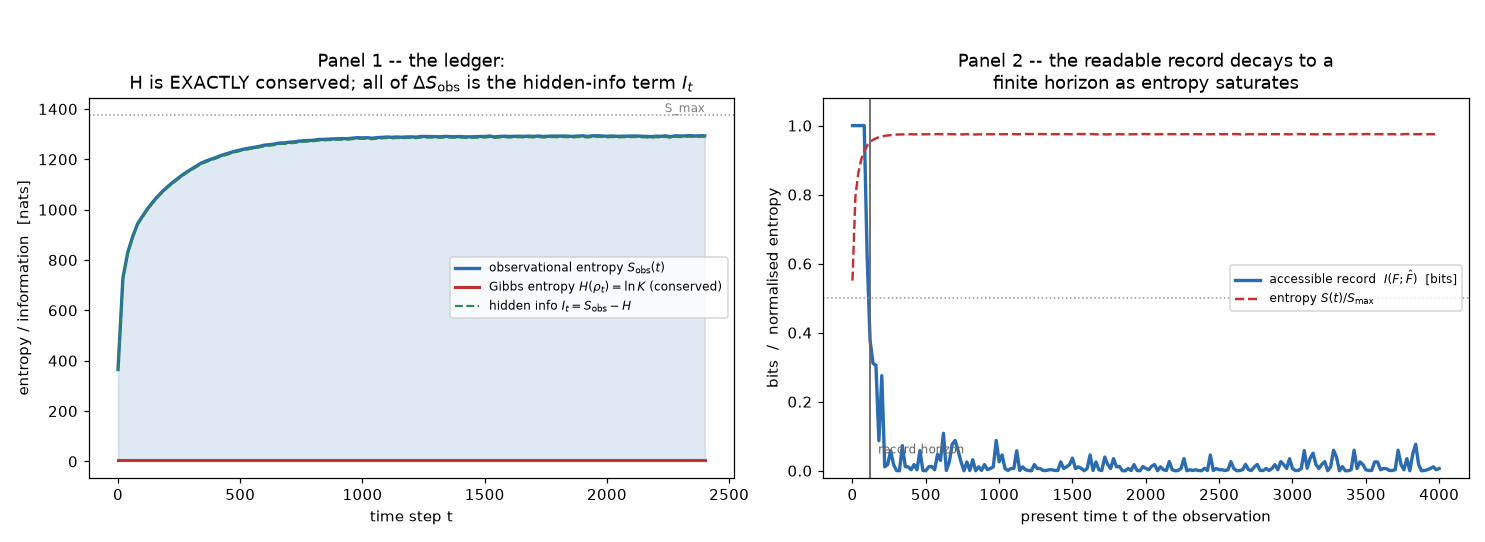
\includegraphics[width=\textwidth]{T7_ledger.png}
\caption{\textbf{Bookkeeping} (bit-reversible lattice gas). Left ($K=64$ worlds, $L=128$,
$b=8$): the fine-grained entropy $H$ of the evolving microstate ensemble is conserved to
machine precision while the observational entropy $S_{\mathrm{obs}}$ rises; by the identity
Eq.~\eqref{eq:ledger} the rise is the hidden-information term $I$. Right (parallel runs,
$K=64$, $L=64$): the accessible record $I(F;\hat F)$ of a planted one-bit fact decays from
$1.000$ to $0.006$ bit as the gas thermalizes.}
\label{fig:ledger}
\end{figure*}

\section{The horizon law for boundary-scale records}
\label{sec:horizon}

Figure~\ref{fig:horizon} shows the baseline measurement. We sweep the scrambling rate
(scatterer fraction $0.15$--$0.42$) with per-condition run lengths chosen so that no
condition is clamped by the simulation window ($T=400$--$2400$ steps, sampling stride
$2$--$6$), five quenched-disorder seeds per condition, $K=40$ worlds per fact class,
$L=64$, $b=4$. Of $25$ runs, $24$ resolve both clocks; one run at the slowest condition
remains censored.

The resolved runs give a proportionality through the origin,
\begin{equation}
\tstar \;=\; 1.08\,\tS, \qquad R^2=0.82,
\end{equation}
over a $7\times$ range of $\tS$ ($26$--$192$ steps). More important than the fit is its
\emph{flatness}: the per-condition ratios are $1.37,\,0.97,\,1.09,\,1.02,\,1.15$ (standard
deviations $0.21$--$0.28$), so the law holds run by run rather than through one leverage
point. (The largest ratio occurs at the fastest condition, where both times are shortest
and the discrete sampling is coarsest relative to them.) A condition-stratified bootstrap
gives a $95\%$ confidence interval $\kap\in[0.91,\,1.24]$; an unconstrained affine fit
$\tstar=a+b\,\tS$ yields an intercept consistent with zero ($a=2.5$, $95\%$ CI
$[-16.2,\,20.4]$) and is not preferred over the one-parameter proportionality (AIC $154.4$
vs $156.3$). The one censored run is qualitatively different, and we diagnose rather than
merely disclose it: its record never degrades at all---$I(F;\hat F)$ dips to $0.855$ bit
and returns to $1.0$, remaining perfectly readable when the run is extended to
$t=12\,000\approx48\,\tS$, while its four sibling seeds cross at $\tstar\approx192$
(Fig.~\ref{fig:anomaly}). The diagnosis: the planted marker is a solid patch, and a fully
occupied (or fully empty) $2\times2$ block is a fixed point of every block rule
\emph{within a single partition}---under the alternating partitions this makes the
\emph{interiors} of solid and void clusters inert while their boundaries can still erode,
and in this one quenched world the erosion stalls. At $t=2400$,
$87\%$ of the class-discriminating signal sits inside the marker boxes and $81\%$ of it on
sites that never move over the measurement window; those frozen sites have occupancy
$0.93$ in each class's own marker box (a solid remnant) and $0.07$--$0.15$ in the opposite
box (a void remnant). The realization is non-ergodic where the record lives \emph{on
every timescale we can observe}: the record's mode shows no relaxation out to
$\tstar\ge12\,000\approx48\,\tS$---a kinetically frozen record, consistent with (though,
absent an invariance proof, not established to be) the protected
$\tau_{\mathrm{mode}}\to\infty$ limit of Eq.~\eqref{eq:modelaw} and of
Sec.~\ref{sec:falsification}, arising here spontaneously from quenched disorder rather
than by engineering. We therefore state the horizon law as holding in $24/25$
realizations, with the exception classified as a frozen-record sector rather than folded
into the fit (as a point value at its lower bound $\tstar\ge T$ it would shift the
through-origin fit to $3.0$ through a single high-leverage point); all its lifetime
statements are lower bounds. Re-deriving both crossings from the stored curves over a grid of gate
conventions quantifies how convention-bound the \emph{number} $\kap$ is:
$\kap=0.87$--$2.83$ for $\theta_S\in\{0.85,0.9\}$, $\theta_M\in\{0.25,0.5,0.75\}$ bit
(a $\theta_S=0.95$ gate lies above the finite-size equilibrium entropy and never resolves).
Each individual crossing moves by $\tau\,\Delta\ln\theta$ as the crossing formula of
Sec.~\ref{sec:mechanism} prescribes---a large effect for the entropy gate because
$0.9\,\Smax$ already sits close to equilibrium---which is why we treat the collapse and
Eq.~\eqref{eq:kappa}, not the numerical $\kap$, as the convention-independent content. The law is also robust in system size: repeating the measurement
with the box and marker scaled together for $L=48$--$128$ ($\tS$ spanning $6\times$) gives
$\kap(L)=0.95,\,0.89,\,0.91,\,1.23$, mean $0.99$, with no systematic drift \cite{repo}.

That $\kap$ sits slightly above unity says only that the $\tfrac12$-bit record threshold is
crossed slightly after the $0.9\,\Smax$ entropy threshold---a statement about conventions
and amplitudes, not physics. The physical content, established next, is that both
observables relax on \emph{one} clock---and Sec.~\ref{sec:modes} shows exactly when that
ceases to be true.

\begin{figure*}
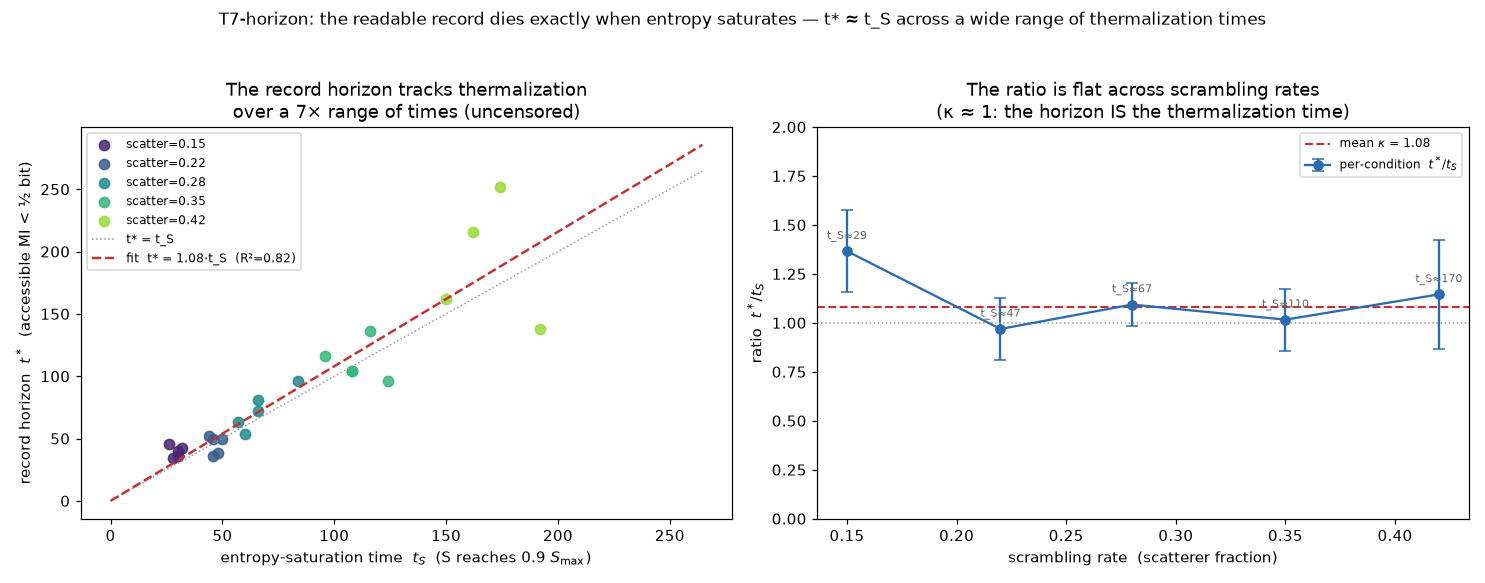
\includegraphics[width=\textwidth]{T7_horizon.png}
\caption{\textbf{The record horizon tracks thermalization for boundary-scale records}
(lattice gas; $5$ scrambling rates $\times$ $5$ disorder seeds; $24/25$ runs resolved,
nothing clamped). Left: $\tstar$ against $\tS$ for all resolved runs; the through-origin
fit gives $\tstar=1.08\,\tS$ ($R^2=0.82$) over a $7\times$ range. Right: the per-condition
ratio $\tstar/\tS$ is flat across scrambling rates---the law holds run by run.}
\label{fig:horizon}
\end{figure*}

\begin{figure*}
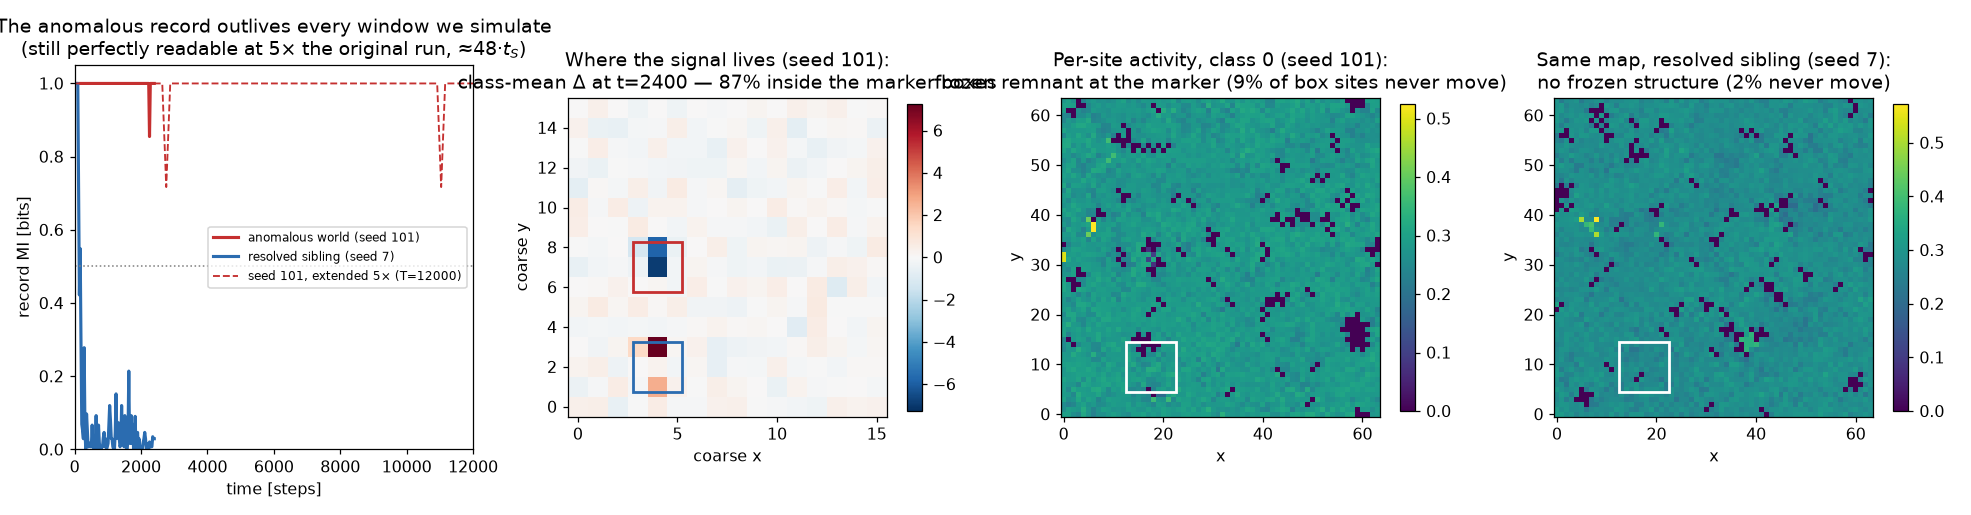
\includegraphics[width=\textwidth]{T7_anomaly.png}
\caption{\textbf{The censored run, diagnosed: a spontaneously frozen record} (scatter
$0.42$, one of five quenched worlds). Left: the anomalous world's record outlives every
window we simulate---still perfectly readable when the run is extended to $5\times$ the
original window ($\approx48\,\tS$)---while a resolved sibling world's record dies on
schedule.
Middle-left: the class-mean coarse difference at $t=2400$ localizes at the two marker
boxes ($87\%$ of $|\Delta|^2$; $81\%$ on never-moving sites). Right two panels: per-site
activity maps; the anomalous world holds a frozen solid remnant of the marker (never-move
sites with occupancy $0.93$ in the own box, $0.07$--$0.15$ in the opposite, initially
empty box), absent in the sibling. A fully occupied or empty $2\times2$ block is a fixed
point of every rule within a single partition, so cluster interiors are inert and a
stalled erosion stores the record for as long as we can measure ($\tstar\ge48\,\tS$;
all lifetime statements are lower bounds)---behaviour consistent with the
$\tau_{\mathrm{mode}}\to\infty$ limit of Eq.~\eqref{eq:modelaw}, realized by quenched
disorder.}
\label{fig:anomaly}
\end{figure*}

\section{A one-slow-mode account}
\label{sec:mechanism}

Why should the two clocks agree? In a finite ergodic system the late-time approach to
equilibrium is dominated by the slowest relaxation mode; for our diffusive lattice gas this
is the largest-wavelength density mode, with lifetime $\tau\sim L^2/D$. In the baseline
construction both observables read that mode. The entropy deficit
\begin{equation}
\mathcal D(t) \;\equiv\; S_{\mathrm{eq}}-S(t) \;\approx\; A_S\,e^{-t/\tau_S}
\end{equation}
measures the large-scale inhomogeneity still to be erased, while the record signal
\begin{equation}
M(t)\;\equiv\;I\!\left(F;\hat F\right)(t) \;\approx\; A_M\,e^{-t/\tau_M}
\end{equation}
\emph{is} the odd (left--right) component of the same relaxation: the planted fact is a
parity of the slowest mode. If one timescale underlies both,
$\tau_M\simeq\tau_S\equiv\tau$, the threshold crossings of Eqs.~\eqref{eq:tS} and
\eqref{eq:tstar} give
\begin{equation}
\tS=\tau\ln\!\frac{A_S}{\theta_S},\qquad
\tstar=\tau_M\ln\!\frac{A_M}{\theta_M},
\end{equation}
with $\theta_S=0.1\,\Smax-\mathcal D_{\mathrm{eq}}$ (the deficit value at the entropy gate,
$\mathcal D_{\mathrm{eq}}$ the finite-size equilibrium deficit) and $\theta_M=\tfrac12$ bit.
Hence
\begin{equation}
\boxed{\;\tstar=\kap\,\tS,\qquad
\kap=\frac{\tau_M}{\tau_S}\,
\frac{\ln(A_M/\theta_M)}{\ln(A_S/\theta_S)}\;}
\label{eq:kappa}
\end{equation}
---a ratio of logarithms of measured amplitudes and chosen thresholds. Equation
\eqref{eq:kappa} organizes the phenomenology: (i) the proportionality itself; (ii) the
flatness of $\kap$ in system size, because $A_S$ scales with $\Smax$ so the logarithm ratio
is size-free; (iii) the substrate dependence of $\kap$ (below: CA $1.08$, hard disks
$1.00$, Clifford $0.79$), because amplitudes and threshold conventions differ between
substrates but enter only through slowly varying logarithms, keeping $\kap$ order one;
(iv) the sensitivity to threshold choices, which enters as a $\tau\,\Delta\ln\theta$
shift of each crossing---modest when a gate sits deep in the relaxing regime, large when it
approaches the equilibrium value (quantified by the gate grid of Sec.~\ref{sec:horizon}).

Figure~\ref{fig:mechanism} tests this account directly ($5$ scrambling rates $\times$ $3$
seeds; both tails fitted per run over their first decaying window,
Appendix~\ref{app:decoder}). The tails are exponential with a \emph{shared} timescale:
$\tau_M/\tau_S=0.92\pm0.30$ across all $15$ runs, flat while the absolute $\tau_S$ varies by
$7.6\times$ ($11$--$84$ steps; condition means $0.76$--$1.16$ with no trend).
Reconstructing the crossing times from each run's fitted $(\tau,A)$ and the thresholds---no
parameters beyond the fitted mode---lands at median error $5\%$ for $\tstar$ and $1\%$ for
$\tS$, with the through-origin $\kap$ reconstructed at $0.98$ against a measured $1.02$ on
the same runs. To make this a prediction rather than an in-sample reconstruction, we also
predict each run's crossings from the tail parameters fitted on the \emph{other} seeds of
its condition (leave-one-out): median errors $19\%$ for $\tstar$ and
$12\%$ for $\tS$. We conclude that, in this construction, record death and
entropy saturation are two threshold crossings of one relaxing mode. What if the record is
\emph{not} written in the slowest mode? That is the decisive question, addressed next.

\begin{figure*}
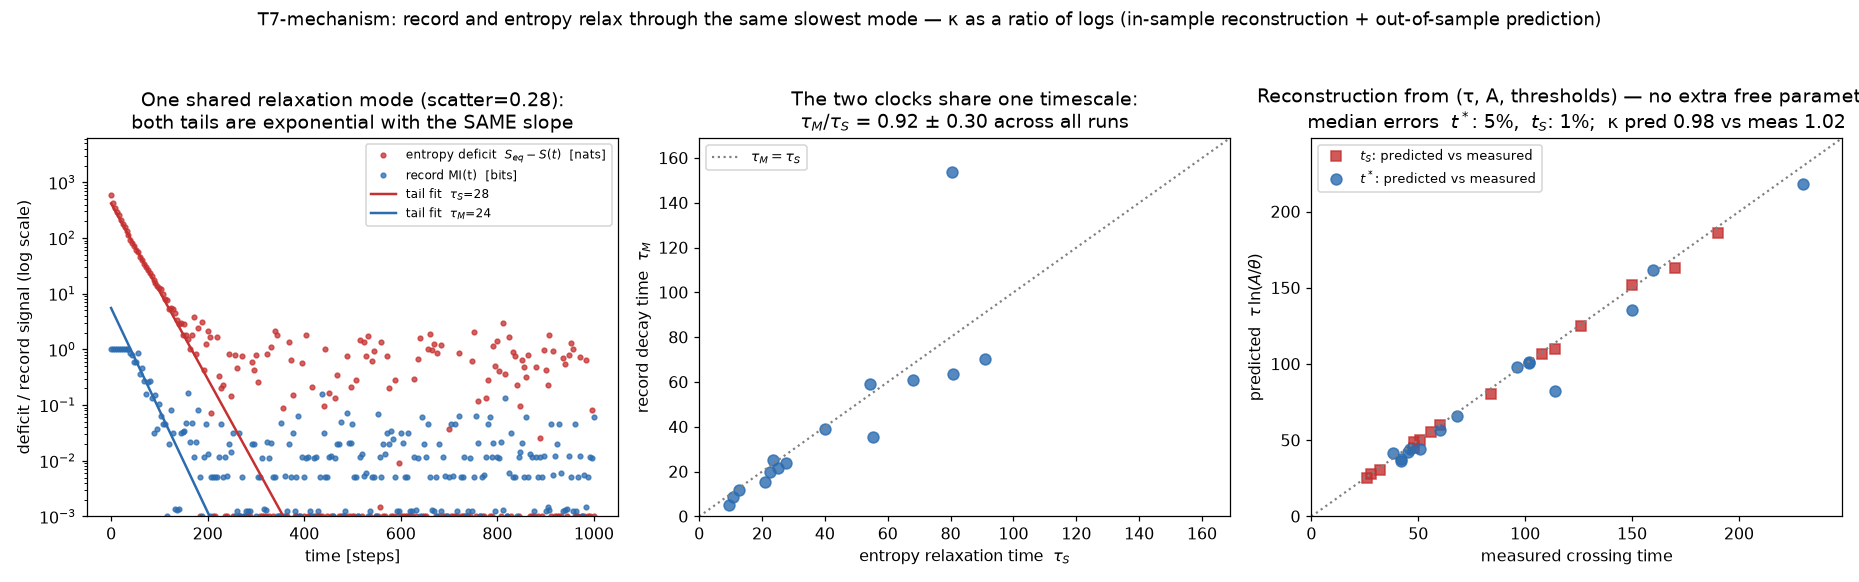
\includegraphics[width=\textwidth]{T7_mechanism.png}
\caption{\textbf{One slow mode, two thresholds} (lattice gas, $5$ scrambling rates
$\times$ $3$ seeds). Left: for one example condition, the entropy deficit
$S_{\mathrm{eq}}-S(t)$ and the record signal $I(F;\hat F)(t)$ on a logarithmic scale; both
tails are exponential with the same slope. Middle: fitted $\tau_M$ against $\tau_S$ for all
runs; the ratio is $0.92\pm0.30$, flat over a $7.6\times$ range of absolute timescales.
Right: reconstruction of both crossing times from the fitted $(\tau,A)$ and the thresholds,
Eq.~\eqref{eq:kappa}: median error $5\%$ ($\tstar$) and $1\%$ ($\tS$); leave-one-out
prediction across seeds performs comparably (see text).}
\label{fig:mechanism}
\end{figure*}

\section{The mode-resolved law: what sets a record's lifetime}
\label{sec:modes}

The account above predicts its own generalization---and its own apparent-counterexample
regime. If a record's lifetime is the threshold crossing of \emph{the mode that carries
it}, then records written at shorter wavelengths must die \emph{before} entropy saturates,
while the entropy clock, which sums over all modes, should not care which record was
planted. ``Record lifetime $=$ thermalization time'' would then be not a general law but
the \emph{supremum} of a mode-resolved law, attained by records written in the slowest
mode. We test this by making the record's wavelength an independent knob.

The blob is prepared with an internal stripe modulation: $2m$ vertical bands, alternately
at densities $0.55$ and $0.35$ (mean $0.45$ as in all other runs), with the one-bit fact
$F$ the stripe \emph{phase} (which band set is dense). The two classes have identical
particle number by construction, and $m=1,2,4,5$ sets the record's wavelength
$\lambda=w/m$. As a reference for each mode's lifetime that involves no \emph{trained}
readout we use the noise-corrected, \emph{label-conditioned} separation power
$\|\Delta(t)\|^2$ (the squared distance between the two classes' mean coarse states, with
the $K$-world sampling floor subtracted---class labels are used, but nothing is fitted),
whose decay time $\tau_{\Delta^2}$ tracks the discriminating signal wherever it drifts;
because
the small-signal mutual information is quadratic in the mode amplitude, the MI tail time
$\tau_M$ should equal $\tau_{\Delta^2}$.

Figure~\ref{fig:modes} shows the result ($K=40$, three disorder seeds per mode):

\begin{itemize}
\item \emph{The entropy clock ignores the record.} $\tS = 98.7,\,96.0,\,94.7,\,93.3$ for
$m=1,2,4,5$---flat to $2.3\%$, as it must be for equal-$N$ states whose coarse entropy is
dominated by the same blob relaxation.
\item \emph{The horizon is mode-matched.} $\tstar = 153,\,57,\,21,\,17$ steps---a
$9\times$ spread at fixed $\tS$. The naive reading of Secs.~\ref{sec:horizon} as ``records
live until thermalization'' is therefore \emph{false in general}: a fine-scale record is
long dead while the gas is still far from saturated.
\item \emph{Each lifetime is its own mode's crossing.} Per mode, the fitted
$(\tau_M,A_M)$ reconstruct $\tstar(m)$ as $\tau_M\ln(A_M/\theta_M) = 154,\,60,\,21,\,17$
---errors of $0.5\%,\,4.7\%,\,1.9\%,\,4.0\%$. The label-conditioned separation-power times agree,
$\tau_M/\tau_{\Delta^2}=0.94,\,0.58,\,0.74,\,1.00$. (The raw $\tstar$-vs-$\tau$ log-log
slope is $1.75$ rather than $1$ precisely because the amplitude logarithm $\ln A_M(m)$
also varies across modes---the lifetime law has both factors.)
\item \emph{The sup form.} Only the blob-scale ($m=1$) record survives to the entropy
clock, $\tstar(1)=1.6\,\tS$; its excess over the baseline $\kap=1.08$ is the amplitude
logarithm of the stronger stripe contrast, again as Eq.~\eqref{eq:kappa} prescribes.
\item \emph{Readout dependence, quantified.} At the slowest mode the three readouts agree
within the logarithmic threshold offsets the mechanism predicts (fixed-template $0.82$,
Gaussian plug-in $1.08$, relative to the trained decoder). For $m\ge2$ the \emph{fixed}
readouts lose the record much earlier ($0.19$--$0.41$ of the trained horizon): a
non-adaptive reader loses a \emph{drifting} fine-scale pattern for physical reasons---an
observation about what it takes to keep reading a record, not a decoding convention.
\end{itemize}

The general law supported by these measurements is
\begin{equation}
\boxed{\;\tstar = \tau_{\mathrm{mode}}
\ln\!\frac{A_{\mathrm{mode}}}{\theta_M}\,,\quad
\max_{\mathrm{relaxing}}\tstar \simeq \mathcal{O}(1)\,\tS\;}
\label{eq:modelaw}
\end{equation}
where the supremum ranges over \emph{relaxing} records in the ergodic sector and is
attained by those written in the slowest thermalizing mode---which is what
boundary-condition facts (``the gas started on the left'') naturally are. The scope
restriction is not pedantry: a non-relaxing mode escapes the bound entirely. The
engineered conservation law of Sec.~\ref{sec:falsification} realizes the
$\tau_{\mathrm{mode}}=\infty$ limit of Eq.~\eqref{eq:modelaw} exactly; the frozen
realization of Sec.~\ref{sec:horizon} is consistent with it on all observed timescales.

\begin{figure*}
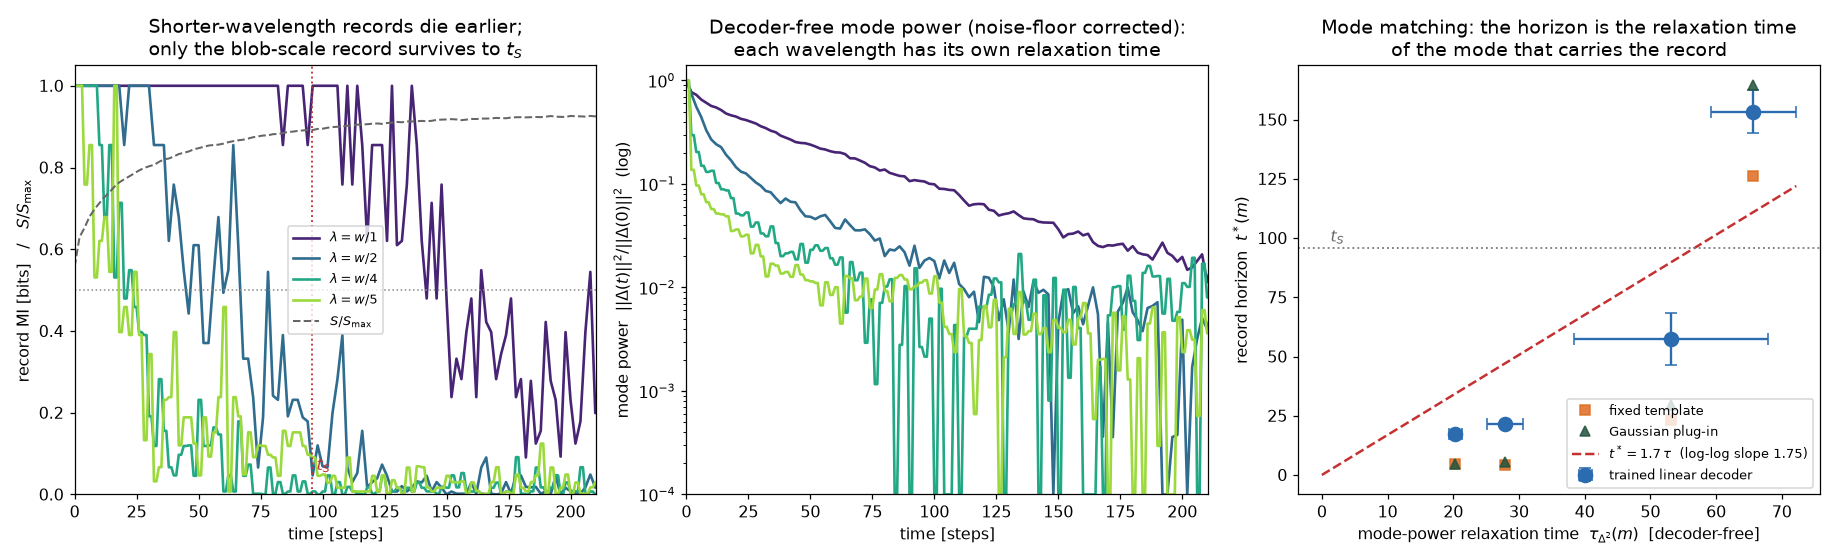
\includegraphics[width=\textwidth]{T7_mode_resolved.png}
\caption{\textbf{The horizon is mode-matched} (lattice gas, stripe-phase records at
wavelengths $\lambda=w/m$, $m=1,2,4,5$; $K=40$, three seeds). Left: record MI for each
wavelength, with $S/\Smax$ (dashed) and $\tS$ marked: shorter-wavelength records die
earlier at fixed entropy clock ($\tS$ flat to $2.3\%$, $\tstar$ spanning $9\times$).
Middle: label-conditioned separation power $\|\Delta(t)\|^2$ on a log scale---each
wavelength has its own relaxation time. Right: $\tstar(m)$ against $\tau_{\Delta^2}(m)$ with the three
readouts; each mode's lifetime is reconstructed by its own $\tau_M\ln(A_M/\theta_M)$ to
$1$--$5\%$ (see text).}
\label{fig:modes}
\end{figure*}

\section{Cross-substrate corroboration}
\label{sec:universality}

A fair objection to Secs.~\ref{sec:horizon}--\ref{sec:mechanism} is that they might
describe an artifact of one substrate---a square lattice gas with quenched scatterers. We
therefore re-ran the two clocks, for boundary-scale records, in two deliberately different
substrates. Given Sec.~\ref{sec:modes}, the meaningful invariant is \emph{mode-matched}
proportionality: when record and entropy relax through the same structure, $\tstar$ and
$\tS$ collapse onto one clock with order-one, convention-bound $\kap$; when the scales are
mismatched, the ratio should (and does) drift.

\subsection{Continuous hard-disk gas}

An event-driven hard-disk gas thermalizes by ballistic crossing rather than lattice
scattering. The mode-matched knob is a \emph{self-similar} size sweep: the low-entropy blob
(and the planted fact) scale with the box, so record and entropy live on the same spatial
scale while the one thermalization time stretches with size. Result (Fig.~\ref{fig:md}):
$\tstar=1.00\,\tS$ over a $5.1\times$ range ($\tS=14$--$73$), per-size
$\kap=1.19,\,1.03,\,0.94,\,0.97,\,1.03$, and both observables collapse onto master curves
under $t/\tS$. The complementary \emph{mode-mismatch control} (Fig.~\ref{fig:mdmismatch})
measures what happens when the scales are deliberately decoupled: the blob (and the fact)
held at fixed absolute size while the box grows leaves the record on a fixed spatial scale
while the entropy clock fills an ever larger volume. Measured: $\tS$ grows $5.1\times$
across the sweep while $\tstar$ varies by only $1.4\times$, so $\kap$ drifts
monotonically from $1.15$ to $0.31$ ($3.7\times$)---and at the smallest box, where the
fixed blob coincides with the self-similar one, $\kap$ agrees with the self-similar
value. The flat law is destroyed exactly when, and only when, the mode matching is
broken: the mode-resolved law of Sec.~\ref{sec:modes}, reasserting itself in a continuous
gas. (This substrate is float-chaotic, so exact values vary at the percent level with the
floating-point environment; an independent re-run of the self-similar sweep on different
hardware gives $\kap=1.04$ with the same flatness \cite{repo}.)

\begin{figure*}
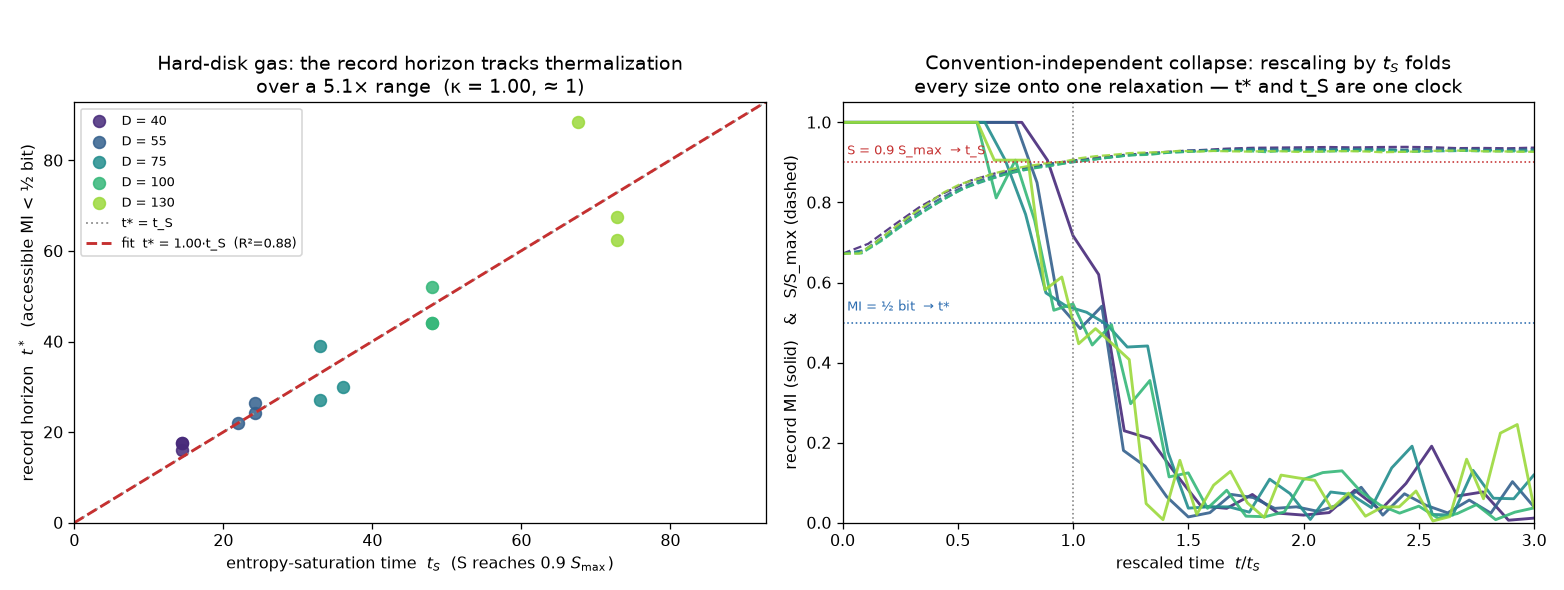
\includegraphics[width=\textwidth]{T7_md_horizon.png}
\caption{\textbf{Cross-substrate corroboration I: continuous hard-disk gas} (self-similar size sweep,
$D=40$--$130$, three seed-ensembles per size). Left: $\tstar$ vs.\ $\tS$;
$\tstar=1.00\,\tS$ over a $5.1\times$ range with flat per-size ratios. Right: rescaling time
by $\tS$ collapses the record MI (solid) and the entropy relaxation (dashed) of every size
onto single master curves. The complementary mode-mismatch control is measured in
Fig.~\ref{fig:mdmismatch}.}
\label{fig:md}
\end{figure*}

\begin{figure*}
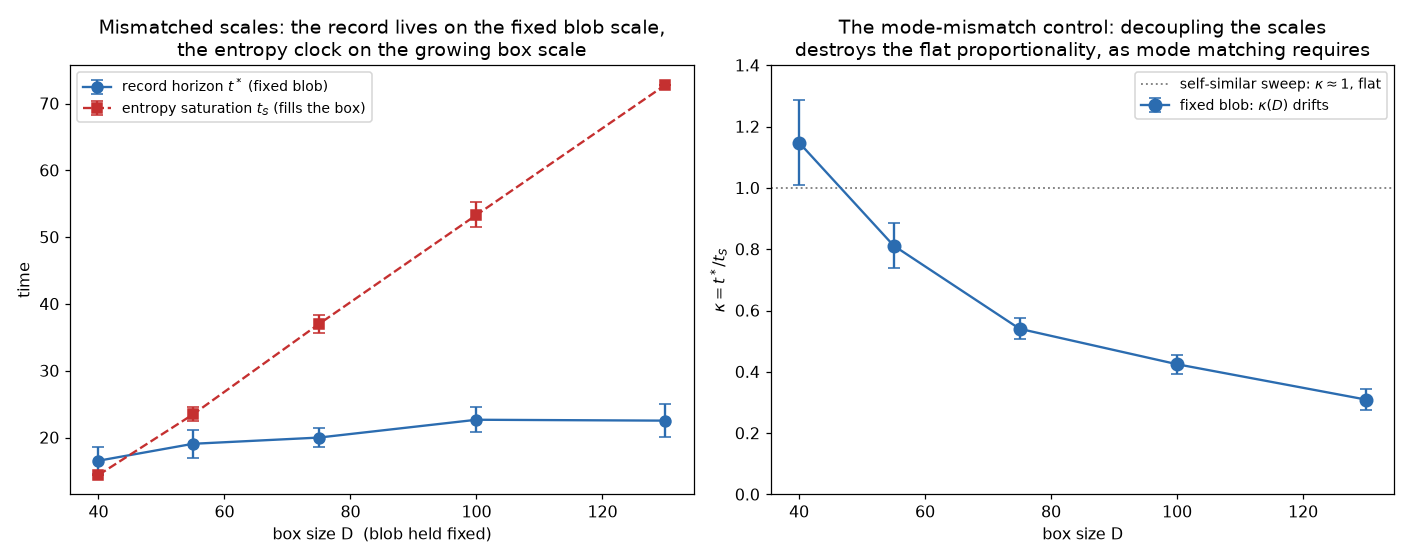
\includegraphics[width=0.86\textwidth]{T7_md_mismatch.png}
\caption{\textbf{The mode-mismatch control} (hard-disk gas; blob and planted fact held at
fixed absolute size while the box grows $D=40$--$130$; three seed-ensembles per size).
Left: the record horizon stays on the fixed blob scale ($\tstar=16.5\to22.5$) while the
entropy clock fills the growing box ($\tS=14\to73$). Right: $\kap=\tstar/\tS$ drifts
monotonically $1.15\to0.31$ instead of staying flat; at $D=40$ the fixed blob coincides
with the self-similar one and $\kap$ matches Fig.~\ref{fig:md}. Decoupling the scales
destroys the flat proportionality exactly as Eq.~\eqref{eq:modelaw} requires.}
\label{fig:mdmismatch}
\end{figure*}

\subsection{Reversible quantum circuits}

The bookkeeping of Sec.~\ref{sec:setup} is natively quantum
\cite{safranek2019a,strasberg2021,zurek2009darwinism}; the lattice gas exercises only its
classical shadow. A Clifford brickwork circuit is unitary---hence exactly reversible---yet
efficiently simulable \cite{gottesman1998,aaronsongottesman2004}, allowing $N=128$ qubits.
Two clocks on the same random circuit: $\tS$ is the half-chain entanglement saturation time
(entanglement first reaches $0.9$ of its late-time Page plateau
\cite{page1993,nahum2017}); $\tstar$ is the time at which a reference qubit's recoverable
record $I(R:\text{local window})$ (window $=N/3$ sites, initially $2$ bits for a maximally
entangled reference) first drops below $1$ bit. Result (Fig.~\ref{fig:clifford}):
$\tstar=0.79\,\tS$ with $R^2=0.95$ over a $6.9\times$ range ($\tS=33$--$229$ layers),
per-size ratios flat at $0.77$--$0.79$ for $N\ge64$, with the same $t/\tS$ collapse. We
note honestly that in this sweep both length scales (half chain, window) are tied to $N$,
so a proportionality is already expected from ballistic information spreading
\cite{nahum2017}; the non-trivial content is the flat order-one value of $\kap$ across
seeds and sizes, the collapse of the full curves, and the contrast with
Sec.~\ref{sec:falsification}, where the identical geometry yields a \emph{diverging} ratio
once the record is protected.

Clifford circuits are simulable precisely because they are non-generic, so we add a
non-Clifford control: a full statevector simulation at $N=8$--$16$ with true von Neumann
entropies, run under random Clifford gates ($\kap=0.89\pm0.32$) and genuinely universal
Haar-random gates ($\kap=0.60\pm0.10$). Both obey the proportional law with order-one
$\kap$; at these small sizes the absolute value is finite-size-suppressed, and the decisive
point is that a universal gate set does not break the law.

\begin{figure*}
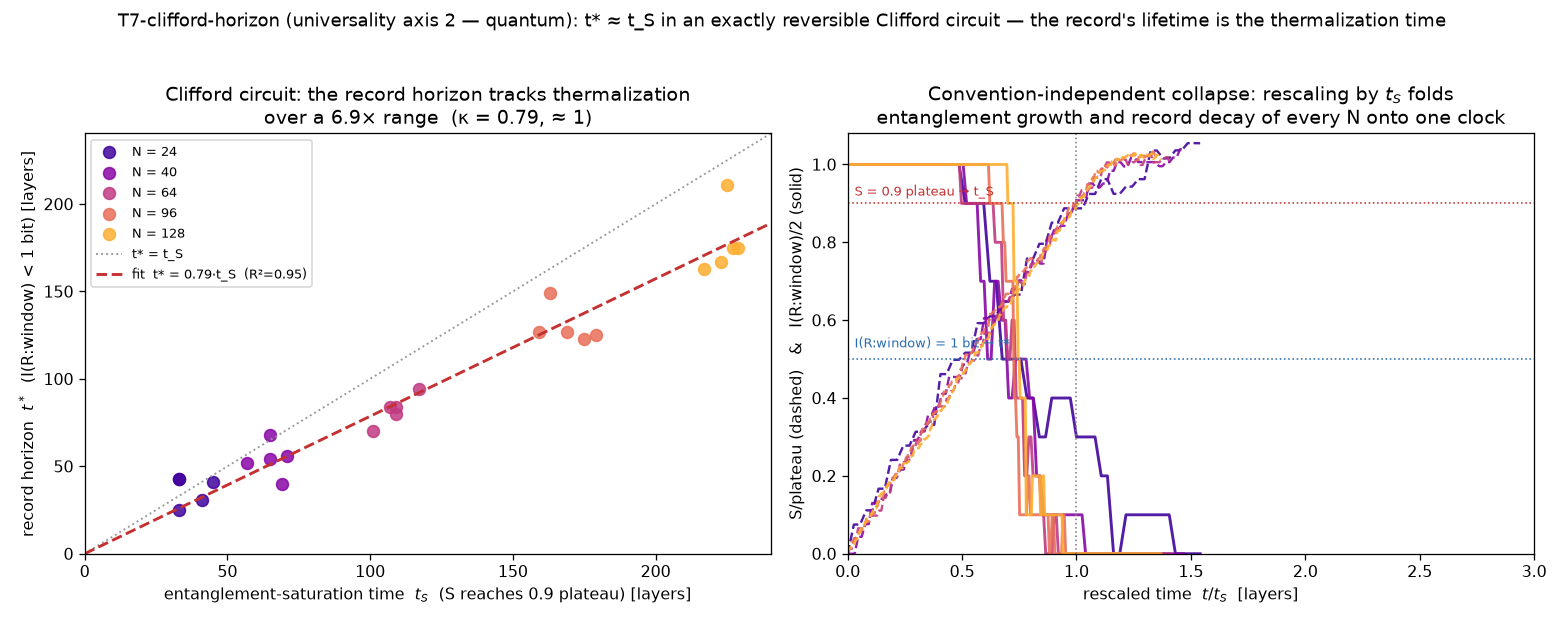
\includegraphics[width=\textwidth]{T7_clifford_horizon.png}
\caption{\textbf{Cross-substrate corroboration II: exactly reversible quantum (Clifford) circuits}
($N=24$--$128$ qubits, five circuit seeds per size). Left: record horizon vs.\
entanglement-saturation time; $\tstar=0.79\,\tS$ ($R^2=0.95$) over a $6.9\times$ range,
per-size ratios flat. Right: $t/\tS$ collapse of entanglement growth (dashed) and record
decay (solid) for all sizes. A statevector control with Haar-random gates (see text)
confirms the behaviour is not a stabilizer artifact.}
\label{fig:clifford}
\end{figure*}

\begin{table}
\caption{The horizon law across substrates (boundary-scale records). $\kap$ is convention-
and substrate-dependent, Eq.~\eqref{eq:kappa}; the law is the flat proportionality.}
\label{tab:kappa}
\begin{ruledtabular}
\begin{tabular}{llll}
Substrate & Dynamics & $\tS$ range & $\kap$ \\
\hline
Margolus CA        & bit-reversible          & $7\times$   & $1.08$ \\
\quad size sweep   & $L=48$--$128$           & $6\times$   & $0.99$ \\
Hard-disk gas      & Hamiltonian             & $5.1\times$ & $1.00$ \\
Clifford circuit   & unitary, $N\le128$      & $6.9\times$ & $0.79$ \\
Haar statevector   & unitary, $N\le16$       & spot        & $0.60(10)$ \\
\end{tabular}
\end{ruledtabular}
\end{table}

\section{Falsifiability: a conservation law decouples the clocks}
\label{sec:falsification}

A law that cannot fail is a definition. Equations~\eqref{eq:kappa} and \eqref{eq:modelaw}
say the horizon tracks the thermodynamic clock only when the record is written in a
\emph{relaxing} mode; the extreme mismatch is a mode that does not relax at all. This
predicts the failure regime exactly: protect the record with a conservation law, and the
two clocks must decouple.

We engineer this in the Clifford substrate (Fig.~\ref{fig:falsification}). A reference qubit
is entangled with a record qubit at the chain end. The bulk scrambles with a random
brickwork (so $\tS$ stays finite), but the bond touching the record qubit is, with
probability $1-p_{\mathrm{break}}$, a protected gate that uses the record only as a control,
conserving $Z_0$ while still broadcasting it; with probability $p_{\mathrm{break}}$ it is a
full scrambling gate. Thus $p_{\mathrm{break}}$ tunes ergodicity at the record. Result
($N=64$, $5N$ layers, four seeds): $\tS$ stays flat across the sweep ($\approx110$ layers,
relative std $0.03$), while
\begin{equation}
\kap(p_{\mathrm{break}})=0.82,\ 0.74,\ 0.80,\ 0.88,\ 1.09,\ \ge1.67,\ \ge2.90
\end{equation}
for $p_{\mathrm{break}}=1,\,0.5,\,0.25,\,0.1,\,0.05,\,0.02,\,0$; at
$p_{\mathrm{break}}\le0.02$ the record outlives every simulated window (censored---the
values quoted are lower bounds), and at $p_{\mathrm{break}}=0$ it is never lost. The horizon
law is therefore \emph{contingent on ergodic scrambling}: a conserved quantity is exactly
what lets a record outlast---or point against---the entropy gradient. This is the extreme
limit of a protected (pointer/code) subspace \cite{zurek2003rmp}; engineered quantum memory
is, in this language, the deliberate construction of horizon-law violations. Mapping this
boundary is what makes the mode-matched law a falsifiable claim about generic dynamics
rather than a tautology of our definitions. And the boundary is crossed spontaneously in
our own data: the diagnosed censored run of Sec.~\ref{sec:horizon} is a quenched world in
which a frozen structure---no engineered gate---stores the record beyond every window we
simulated ($\ge48\,\tS$).

\begin{figure*}
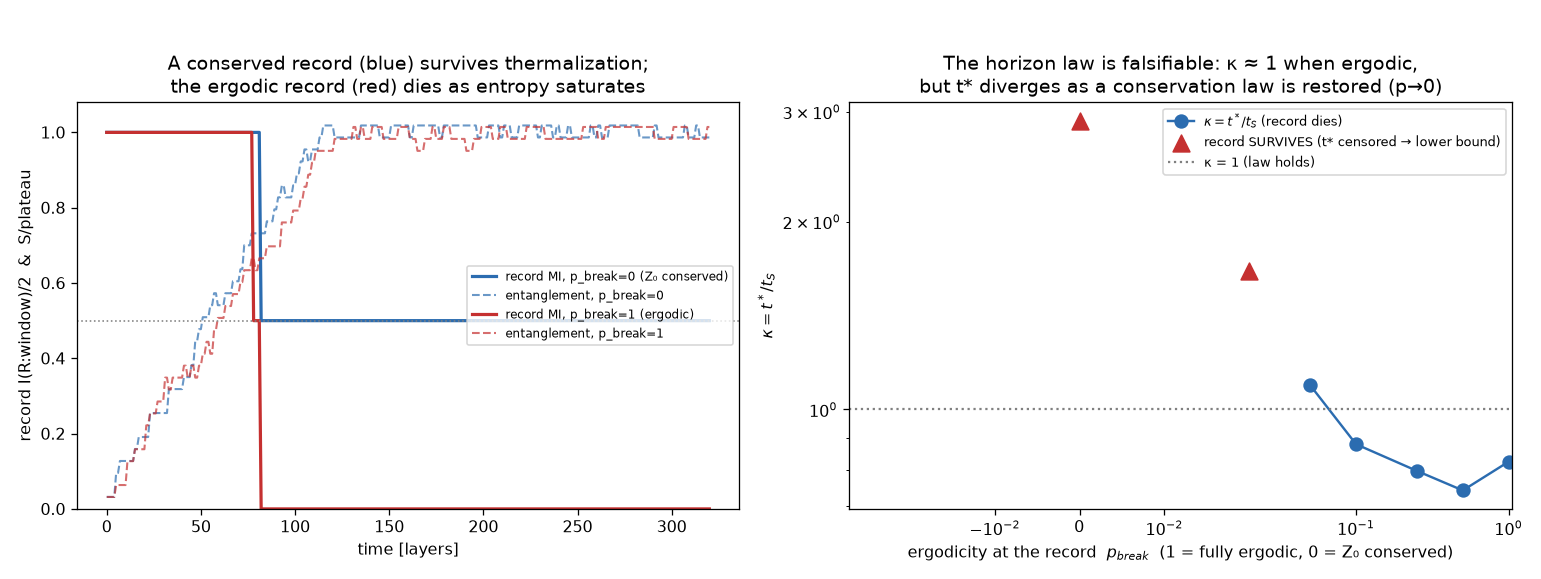
\includegraphics[width=\textwidth]{T7_clifford_falsification.png}
\caption{\textbf{The law fails where it must} (Clifford chain, $N=64$; a tunable
$Z_0$-conserving gate protects the record with probability $1-p_{\mathrm{break}}$). Left:
example trajectories---under full scrambling the record dies as entanglement saturates,
while the protected record survives arbitrarily long although the bulk thermalizes
identically. Right: $\kap=\tstar/\tS$ against $p_{\mathrm{break}}$; the ratio is order one
in the ergodic regime and diverges (censored points are lower bounds) as the conservation
law is restored, while $\tS$ stays flat.}
\label{fig:falsification}
\end{figure*}

\section{Redundancy: classical Darwinism and its scaling}
\label{sec:redundancy}

How is the record stored while it lives? Following the quantum Darwinism program
\cite{zurek2009darwinism,blumekohout2006,riedel2012risefall} we measure the
partial-information profile of the classical record: the mutual information $I_f$ recovered
by decoders restricted to random fractions $f$ of the coarse cells, and the effective
redundancy $R_\delta=1/f_\delta$, where $f_\delta$ is the smallest fraction achieving
$(1-\delta)I_{\max}$ (we use $\delta=0.1$; $R_\delta$ counts recoverable fragments, without
asserting their mutual conditional independence). Near the boundary the profile has the
classical plateau shape: $10\%$ of the cells already recover $89\%$ of the record, and
$R_\delta\approx8$--$10$, collapsing to $R_\delta=1$ at the horizon \cite{repo}---the
classical analogue of the rise and fall of redundancy \cite{riedel2012risefall}.

\subsection{Scaling with environment size}

A diffusion/signal-to-noise argument fixes the ideal scaling. Growing the system
self-similarly (box $L$ up at fixed cell size $b$, marker scaled with $L$) adds
\emph{equivalent} fragments: each added cell is an equally informative detector of the
planted parity near the boundary, so ideally one new recoverable copy per added fragment,
$R\propto N$ with $N=(L/b)^2$, i.e.\ $\alpha=1$ (ideal classical Darwinism). Refining the
grid instead ($b$ down at fixed $L$) multiplies fragments while dividing the per-fragment
signal, so $\alpha<1$ is expected---an SNR-confounded control.

Figure~\ref{fig:redundancy} shows the measured scaling over $N=144$ to $16{,}384$
($L=48$--$512$, six disorder seeds): $R$ climbs from $7.3$ to $438$. A power law over the
full range gives $\alpha=0.88$; the finite-size-free tail ($L\ge128$) gives
$\alpha=0.91\pm0.05$; and two independent extrapolations (a cutoff sweep in $N_{\min}$ and a
correction fit $R=A\,N^{\alpha}(1+c/N)$, mutually agreeing) give
\begin{equation}
\alpha_\infty = 0.92\pm0.04,
\end{equation}
$2.2\sigma$ below the ideal value---ideal Darwinism \emph{supported but not certified} at
accessible sizes. This quote is deliberately conservative: the data cannot distinguish the
form of the finite-size correction (near-identical residuals), and the physically motivated
$c/\sqrt N$ correction (the marker spans $\propto L=b\sqrt N$ cells) gives
$\alpha_\infty=0.95\pm0.07$, while $c\,N^{-1/4}$ gives $1.00\pm0.12$
(Appendix~\ref{app:extrapolation}). Meanwhile the SNR-confounded refinement sweep stays at
$\alpha=0.71$: the two ways of growing the environment separate cleanly, exactly as the
argument predicts.

\subsection{The quantum broadcast limit}

In the stabilizer substrate we compare Zurek's dichotomy directly (Fig.~\ref{fig:qdarwin}):
a pointer bit \emph{broadcast} into $N_E$ environment qubits (decoherence-type dynamics)
yields a flat partial-information plateau---any fragment carries the full classical
record---and $R_\delta=N_E$ exactly across $N_E=8$--$128$, i.e.\ $\alpha=1$: ideal
Darwinism, realized in the noiseless limit. The same pointer under \emph{scrambling}
dynamics is encoded rather than broadcast: the partial-information profile becomes a step
at half the environment and $R_\delta\approx1$. Since perfect discrete copying has no SNR
loss, the broadcast model reaches the exponent the diffusive classical lattice only
approaches; this is \emph{consistent with}---though, being a different model, it cannot by
itself prove---the classical shortfall being a signal-to-noise and finite-size effect
rather than a limit of the redundancy principle. (We note honestly that broadcast
redundancy is fragile: a few scrambling layers collapse $R_\delta$ toward $1$ well before
the entropy horizon---redundant, multi-observer accessibility dies earlier than the
single-copy record of Fig.~\ref{fig:clifford}, consistent with \cite{riedel2012risefall}.)

\begin{figure*}
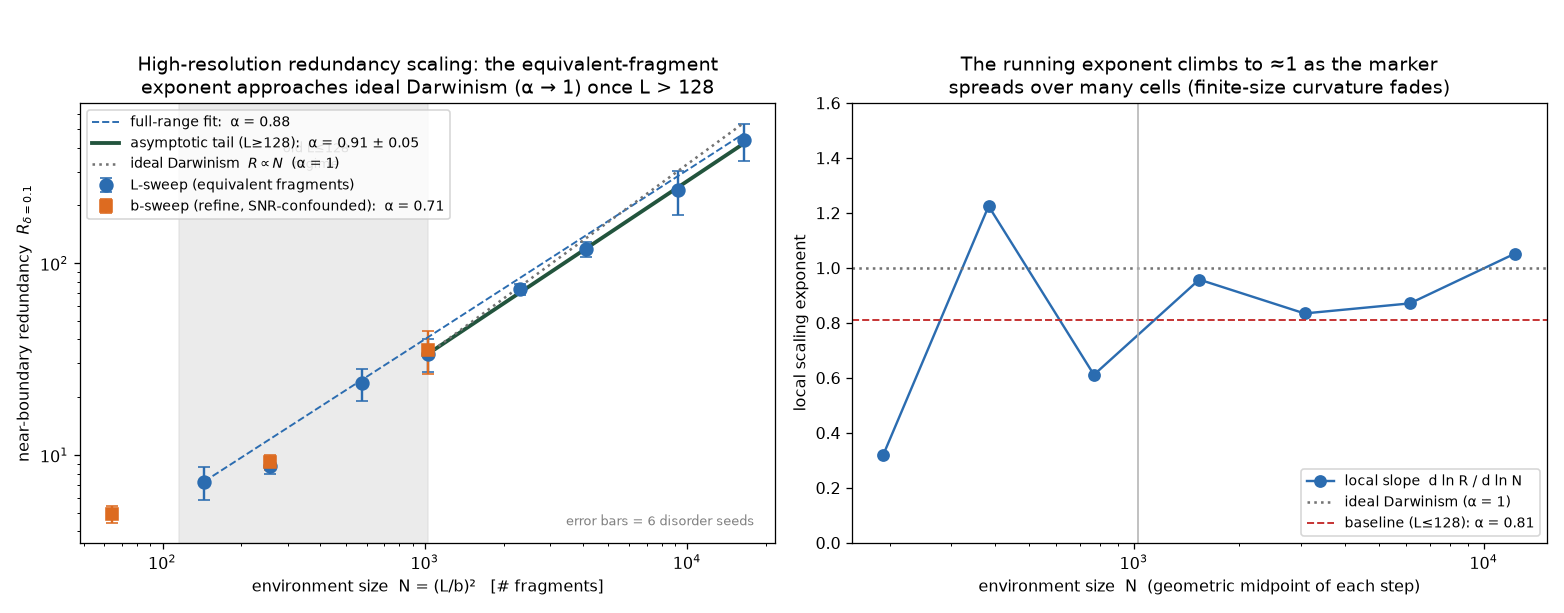
\includegraphics[width=\textwidth]{T7_redundancy_scaling_hires.png}
\caption{\textbf{Redundancy scaling toward ideal Darwinism} (lattice gas, equivalent-fragment
sweep $L=48$--$512$, i.e.\ $N=(L/b)^2$ up to $16{,}384$; six disorder seeds). Left:
near-boundary effective redundancy $R_{\delta=0.1}$ vs.\ $N$; the full-range exponent is
$0.88$, the $L\ge128$ tail $0.91\pm0.05$ (extrapolating to $\alpha_\infty=0.92\pm0.04$,
conservatively; see text), while the SNR-confounded refinement sweep stays at
$\alpha=0.71$. Right: the local slope $d\ln R/d\ln N$ climbs to $\approx1$ at the largest
sizes as the small-$L$ curvature fades.}
\label{fig:redundancy}
\end{figure*}

\begin{figure*}
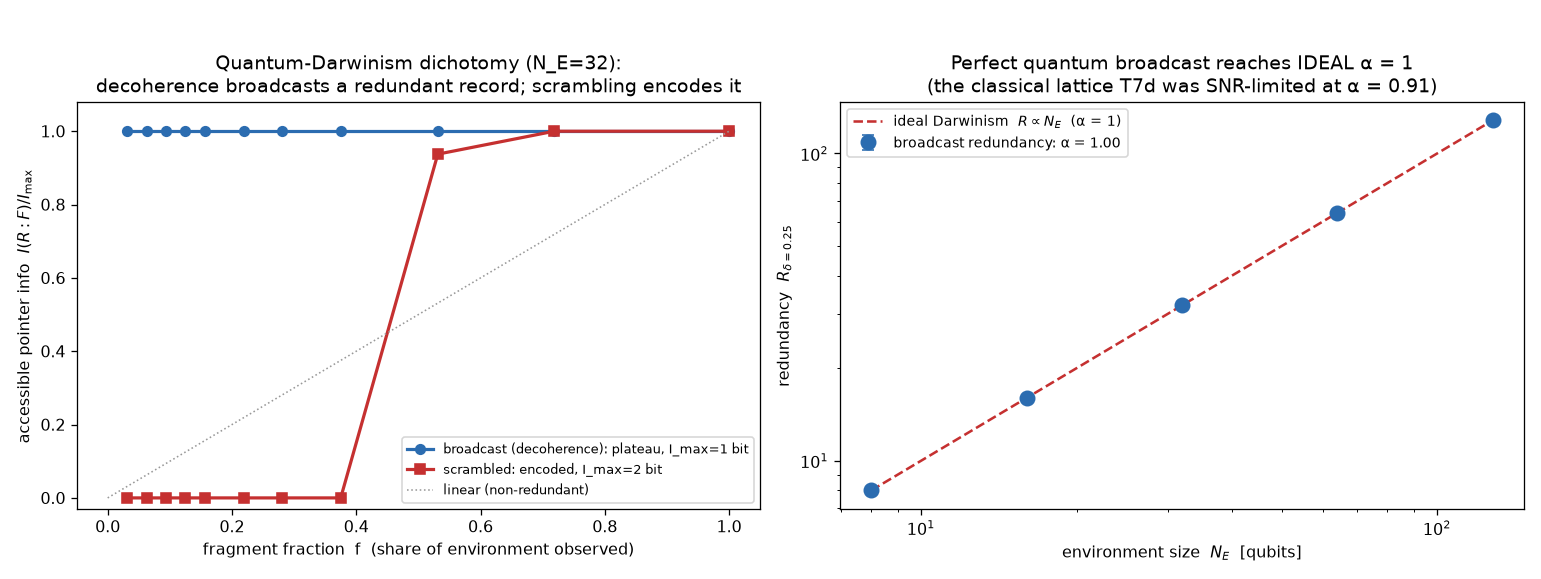
\includegraphics[width=\textwidth]{T7_clifford_darwinism.png}
\caption{\textbf{Quantum Darwinism in the reversible circuit substrate.} Left:
partial-information profiles for a pointer bit broadcast into the environment (flat plateau:
any small fragment carries the record) versus scrambled into it (step at half the
environment: the record is encoded, not redundant). Right: effective redundancy of the
broadcast record scales as $R_\delta=N_E$ exactly ($\alpha=1$, $N_E=8$--$128$)---the ideal
limit the classical lattice approaches from below.}
\label{fig:qdarwin}
\end{figure*}

\section{Discussion}
\label{sec:discussion}

\subsection{What has been established}

Within exactly reversible model dynamics prepared at a low-entropy boundary: (i) the growth
of coarse entropy is, by the observational-entropy identity, the growth of information
hidden from the coarse observer, with the fine-grained entropy conserved to machine
precision, while planted records decay to zero in parallel; (ii) for boundary-scale
records the operational horizon tracks the entropy-saturation time, $\tstar=\kap\,\tS$
with order-one $\kap$, flat across dynamics rates and sizes and reproduced across three
substrates (Table~\ref{tab:kappa}); (iii) a one-slow-mode account reproduces the crossings
in-sample and out-of-sample and reduces $\kap$ to a ratio of logarithms; (iv) resolving
records by wavelength shows the general law is \emph{mode-matched},
Eq.~\eqref{eq:modelaw}: the entropy clock is record-independent while lifetimes span an
order of magnitude, each set by its own mode's relaxation and amplitude, with
``lifetime $=$ thermalization time'' as the supremum attained by slowest-mode records;
(v) the law fails precisely when the record is stored in a non-relaxing structure---the
$\tau\to\infty$ limit of the same statement---whether engineered (a conservation law,
Sec.~\ref{sec:falsification}) or spontaneous (the diagnosed frozen realization,
Sec.~\ref{sec:horizon}); (vi) records are stored redundantly, with an
effective-redundancy scaling that approaches ideal classical Darwinism and attains it in
the noiseless quantum broadcast.

Taken together, these results sharpen the qualitative account of the memory arrow
\cite{reichenbach1956,wolpert1992,mlodinowbrun2014,rovelli2020memory}. Mlodinow and Brun
argued that a robust record-forming system must sit on the entropy-increasing side of the
gradient \cite{mlodinowbrun2014}; Rovelli, that memories degrade as the system thermalizes
\cite{rovelli2020memory}. Our measurements supply the quantitative structure: \emph{which}
records last is set by mode matching; the most durable record's lifetime is the
thermalization time itself; objectivity while alive is redundancy; and outliving the
gradient requires a non-relaxing structure. In our data that happened two ways: by
engineered protection (Sec.~\ref{sec:falsification}), and unbidden, in one of $25$
disordered realizations, by spontaneous freezing (Sec.~\ref{sec:horizon})---nature does
occasionally build its own memory protection, and when it does, the record decouples from
the thermodynamic clock for as long as we can follow it. In companion experiments in the same testbed \cite{repo}, the
\emph{direction} of record accumulation flips with the sign of the entropy gradient
(including for facts injected mid-run, realizing Reichenbach's fork asymmetry), completing
the picture: direction, lifetime, and storage of memory are all read off the gradient.

\subsection{What has \emph{not} been shown}

First and fundamentally, nothing here derives the arrow of time: every run assumes the
low-entropy boundary. This is not a defect of the testbed but a theorem-level wall for any
time-symmetric dynamics \cite{loschmidt1876,price1996}; our exactly reversible substrate
makes it vivid, since entropy grows in \emph{both} time directions away from the boundary
state \cite{repo}. The mystery of the Past Hypothesis is used, not dissolved. (An
exploratory companion experiment relocates the posit in the spirit of Carroll and Chen
\cite{carrollchen2004}---a \emph{small} early volume plus expansion, rather than a
fine-tuned microstate, sustains an unbounded two-headed entropy valley from a single bounce
microstate evolved in both time directions---but the relocated question, why the volume was
small, remains as open as the original \cite{repo}.)

Second, $\tstar$ is operational: the horizon of an explicit decoder class, hence a lower
bound on the accessible-information horizon. We quantified its readout dependence
(Sec.~\ref{sec:modes}) but have not computed the information-theoretic horizon itself.
Third, $\kap$'s numerical value is convention-laden; only the shared relaxation, its mode
structure, and the collapses are physics. Fourth, the classical redundancy exponent is
supported at, but not certified to, the ideal value ($\alpha_\infty=0.92\pm0.04$
conservatively, up to $1.00$ under equally consistent extrapolation forms); certification
would require another decade in $N$. Fifth, all claims are about the model classes
simulated here---though three substrates, a mode-resolved mechanism, and a mapped failure
boundary argue that mode-matched horizons are a generic property of ergodic reversible
information dynamics rather than an artifact of any one model.

\subsection{Outlook}

Three extensions seem most valuable. (i) A quantitative tie of the mode times to
transport: the account predicts $\tau(\lambda)\propto\lambda^2/D$ in the hydrodynamic
regime, with $D$ set by the scatterer density; our measured $\tau_{\Delta^2}(m)$ decays
more slowly with $m$ than $\lambda^2$ at these sizes, and mapping that crossover would
express the horizon entirely in transport coefficients. (ii) Computing the
information-theoretic horizon (or tighter decoder hierarchies) to close the operational
gap. (iii) In the corroboration direction \cite{repo}: conditioning equilibrium
fluctuations on reproducing one half of a record and testing whether the other half
corroborates would quantify why multiple independent records justify belief in a real
low-entropy past---Reichenbach's common cause as a measurable statement.

\begin{acknowledgments}
All simulations, per-experiment numerical verdicts, the scripts generating every figure,
and per-run data for the core experiments (\texttt{data/}) are openly available
\cite{repo}.
\end{acknowledgments}

\appendix

\section{The bit-reversible substrate}
\label{app:model}

The Margolus automaton partitions the $L\times L$ periodic grid into $2\times2$ blocks, with
the partition offset alternating each step. Each block is updated by a bijective lookup
table acting on its $16$ possible occupancies; the composition of bijections is a bijection,
so the global map is exactly invertible, and running the inverse tables in reverse order
returns the initial bitstring exactly (verified bit-for-bit \cite{repo}). A
quenched fraction (the scrambling knob) of blocks applies a rotation rule; the remainder
apply the identity-preserving collision rule. Initial low-entropy states confine all
particles to a width-$w$ blob at density $\rho$ ($w=40$, $\rho=0.45$, $L=64$, $b=4$ for the
horizon experiments), with microstates sampled microcanonically. The hard-disk companion is
an event-driven elastic-disk gas in a square box with specular walls; between collisions the
flight is exact, so the only irreversibility is floating-point.

\section{Records, decoders, and tail fits}
\label{app:decoder}

The baseline fact $F$ places a marker of identical particle number on the left or right of
the blob, so the classes share every conserved quantity; the mode-resolved facts of
Sec.~\ref{sec:modes} are stripe phases at wavelength $w/m$, also with identical $N$ by
construction. For each class, $K$ microstates are evolved through the same quenched
disorder ($K=40$ for the horizon and mode sweeps, $64$ for the ledger). At each sample time
the coarse occupancy vectors of half the worlds train a nearest-centroid linear readout
$\hat F$; $I(F;\hat F)$ is computed from the held-out confusion matrix. This makes $\tstar$
an \emph{operational} horizon: the time past which this readout of the present coarse state
retains less than half a bit about the fact. The alternative readouts of
Sec.~\ref{sec:modes} are (a) an untrained fixed-template decoder (the sign of the
projection onto the $t=0$ stripe pattern) and (b) a Gaussian plug-in mutual information on
the held-out one-dimensional stripe projection, with the finite-sample separation bias
$\sigma^2(2/n)$ subtracted so the estimate decays to zero rather than to a sampling floor.
The label-conditioned separation power is
$\|\Delta(t)\|^2=\|\bar V_0(t)-\bar V_1(t)\|^2$ minus its $K$-world sampling floor,
where $\bar V_c$ is the class-mean coarse state (class labels enter; no decoder is
trained).

For the ledger, an ensemble of $K$ equiprobable microstates gives $H=\ln K$ exactly under
bijective evolution, while the coarse observer assigns the observational entropy
\cite{safranek2019a,safranek2021intro}; the hidden-information term of
Eq.~\eqref{eq:ledger} is the difference, computed exactly from the evolving ensemble.

For the tail fits, the equilibrium deficit $\mathcal D_{\mathrm{eq}}$ (mean of the last
$15\%$ of each run) is subtracted before fitting; each tail is fitted by ordinary least
squares on $\ln y$ over its first decaying crossing of a fixed window ($[0.04,0.5]$ of the
initial deficit for $\mathcal D$; $[0.04,0.6]$ bit for $M$), which excludes the estimation
floor that follows the record's death.

\section{Stabilizer methods}
\label{app:stabilizer}

Clifford states are tracked by the binary check matrix of their stabilizer group (phases
dropped; they do not affect entanglement). Gates act as column operations
\cite{gottesman1998,aaronsongottesman2004}. The entanglement entropy of a region $A$ is
$S_A=\mathrm{rank}_{\mathbb F_2}(G|_A)-|A|$ ebits \cite{fattal2004}, and mutual informations
follow from $I(A{:}B)=S_A+S_B-S_{AB}$. Brickwork layers apply independent random two-qubit
Cliffords (random single-qubit words interleaved with CNOTs in both directions) to
alternating bonds; this drives contiguous regions to volume-law (Page) entanglement
\cite{page1993,nahum2017}. The protected gate of Sec.~\ref{sec:falsification} uses the
record qubit only as a control, conserving $Z_0$. The statevector control applies exact
$4\times4$ unitaries (Haar-random via QR of complex Gaussians, or random Clifford words) and
computes von Neumann entropies from Schmidt spectra.

\section{Extrapolation of the redundancy exponent}
\label{app:extrapolation}

Two estimators of the asymptotic exponent agree: (A) a cutoff sweep, fitting
$\alpha_{\mathrm{eff}}(N_{\min})$ on $N\ge N_{\min}$ and extrapolating linearly in
$1/N_{\min}\to0$ (giving $0.918$); and (B) a correction fit
$\ln R=c_0+\alpha_\infty\ln N+c_1 N^{-p}$ with seed-bootstrapped errors. For $p=1$:
$\alpha_\infty=0.922\pm0.036$; $p=\tfrac12$: $0.947\pm0.067$; $p=\tfrac14$:
$1.001\pm0.124$---with statistically indistinguishable residuals (RSS
$0.060/0.063/0.064$), so the main text quotes the most conservative value. The local slope
$d\ln R/d\ln N$ reaches $0.96$--$1.05$ across the largest size steps.

\bibliography{refs}

\end{document}
